\section{Specialized hardware generation with fusion}

As has already been mentioned, we utilize distillation to provide fusion for routines written in a simple functional programming language and utilize FHW compiler, which is able to translate any Haskell program into SystemVerilog and eventually into bitcode for  FPGA. This section discusses how the gap between the distiller language and Haskell was closed, what issues in FHW were found and how they were solved. Also the section describes data structures being used for which fusion via distillation works well.


\subsection{Distiller}

The distiller from~\cite{distillation} operates on programs written in \texttt{.pot} language: a simple call-by-name functional language. Its syntax resembles the one of Haskell, but it encloses the arguments of a constructor in parentheses and separates them with a comma to make parsing easier. In order to emit Haskell, the pretty-printer prints such constructors correspondingly and maintains correct indentation for case alternatives, which are originally separated by \texttt{|} in \texttt{.pot}. With such modifications, it is possible to emit Haskell code from \texttt{.pot} programs and eventually pass them into FHW compiler. It is worth noting that \texttt{.pot} assumes a Hindley-Milner type system, but its implementation is untyped; thus the emitted program should be extended by hand to contain proper type definitions and annotations where needed to eliminate unnecessary typeclasses.

Another issue is that the distiller originally produced duplicated functions during residualization. Such functions increase the size of the generated hardware significantly for reasonable examples and make translation into hardware more complex. The functions are filtered to contain only non-duplicates. Since functions use De Bruijn indexes for bound variables, functions are considered to be duplicates if their bodies are equal after we replace each recursive call in one function with the name of the other function.

\subsection{FHW}

Unlike~\cite{Edwards2019FHWP}, which utilized C++ Verilator simulation, we use Xilinx Vivado to both simulate the generated SystemVerilog and to synthesize it. It allows to better estimate design and memory transferring overheads.

Initially, generated hardware did not work in Vivado simulation due to the multiple driving of \texttt{initial} blocks, which are also not synthesizable. Such blocks were replaced with a \texttt{reset} signal. The dataflow network works under valid-ready protocol, and memory output had to be invalidated to prevent the propagation of undefined signals. Such outputs are invalidated on the positive edge of the reset signal.

After that, it appeared that the compiler could not handle examples with sparse linear algebra routines due to the limited maximum number (64) of inputs in merge actors. For each merge actor in the dataflow there is a sum datatype with the number of fields equal to the number of merge inputs to be able to correctly type each merge and to identify the chosen input to pass that choice to another actor: demux, fork or mux. Such datatypes are recursively split until every datatype satisfies the restriction. The inputs of a merge are also split and a new layer of merge actors is added on top, as it could be seen in figure~\ref{fig:compressChoice} where the limit is 2 while the original input size is 4; consuming actor is split accordingly. Similar procedure is applied for datatypes that arise during lowering passes of FHW, for example, if the defunctionalization pass introduces more than 64 constructors in the corresponding datatype. An example of such step could be seen in listing~\ref{lst:split}, if we suppose that maximum supported number of alternatives is 4.

\begin{listing}
\begin{center}
\begin{minted}{Haskell}

data Cont = C_1 | C_2 | C_3 | C_4
-- transformed into
data LeftCont = C_1 | C_2
data RightCont = C_3 | C_4
data Cont = LeftCont | RightCont

\end{minted}
\caption{Data type split step}
\label{lst:split}
\end{center}
\end{listing}


\begin{figure}
    \centering
    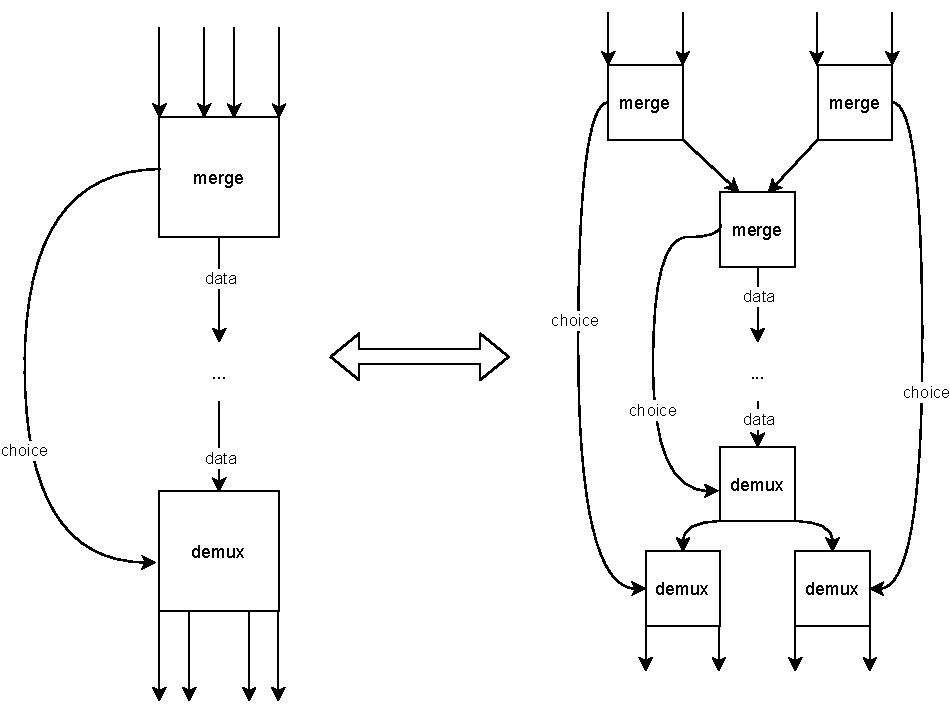
\includegraphics[width=0.8\textwidth]{figures/compressChoice.pdf}
    \caption{Merge split}
    \label{fig:compressChoice}
\end{figure}

\subsection{Data types}

The success of sparse linear algebra functions fusion depends on the compressed representation being used. Our choice here is quadtree representation~\cite{qtree}. It provides a reasonable compression rate compared to traditionally used formats, e.g., coordinate format, or compressed sparse row representation~\cite{GAILLA}, consuming 1.5x more memory on average in our experiments, although memory consumption grows logarithmically with the dimensions of a matrix. Also, it allows to express algorithms in a divide and conquer manner leaving indexing implicit, which facilitates fusion. The representation simply recursively splits the matrix into submatrices until the size of 1x1 or until the submatrix is empty. Thus it encodes only matrices with the size of power of 2, but any matrix could be extended with zeroes to fit the size requirement. An example of such representation could be seen in figure~\ref{fig:qtree}, where a matrix with 4 non-zero entries is depicted. Dashed squares represent either submatrix with only zero entries or zero entry. A procedure of getting a quadtree representation from coordinate format could be found in~\cite{matrix-rep}. Since the representation is constructive, it is possible to utilize dependent type programming techniques to, for example, specify correct by construction routines or use rewrite rules for matrix relations to optimize routines, following the approach of~\cite{typeyourmatricesforgreatgood}. Next, we use terms tree, quadtree or matrix interchangeably: they all mean a sparse matrix representation via quadtree. 

\begin{figure}
    \centering
    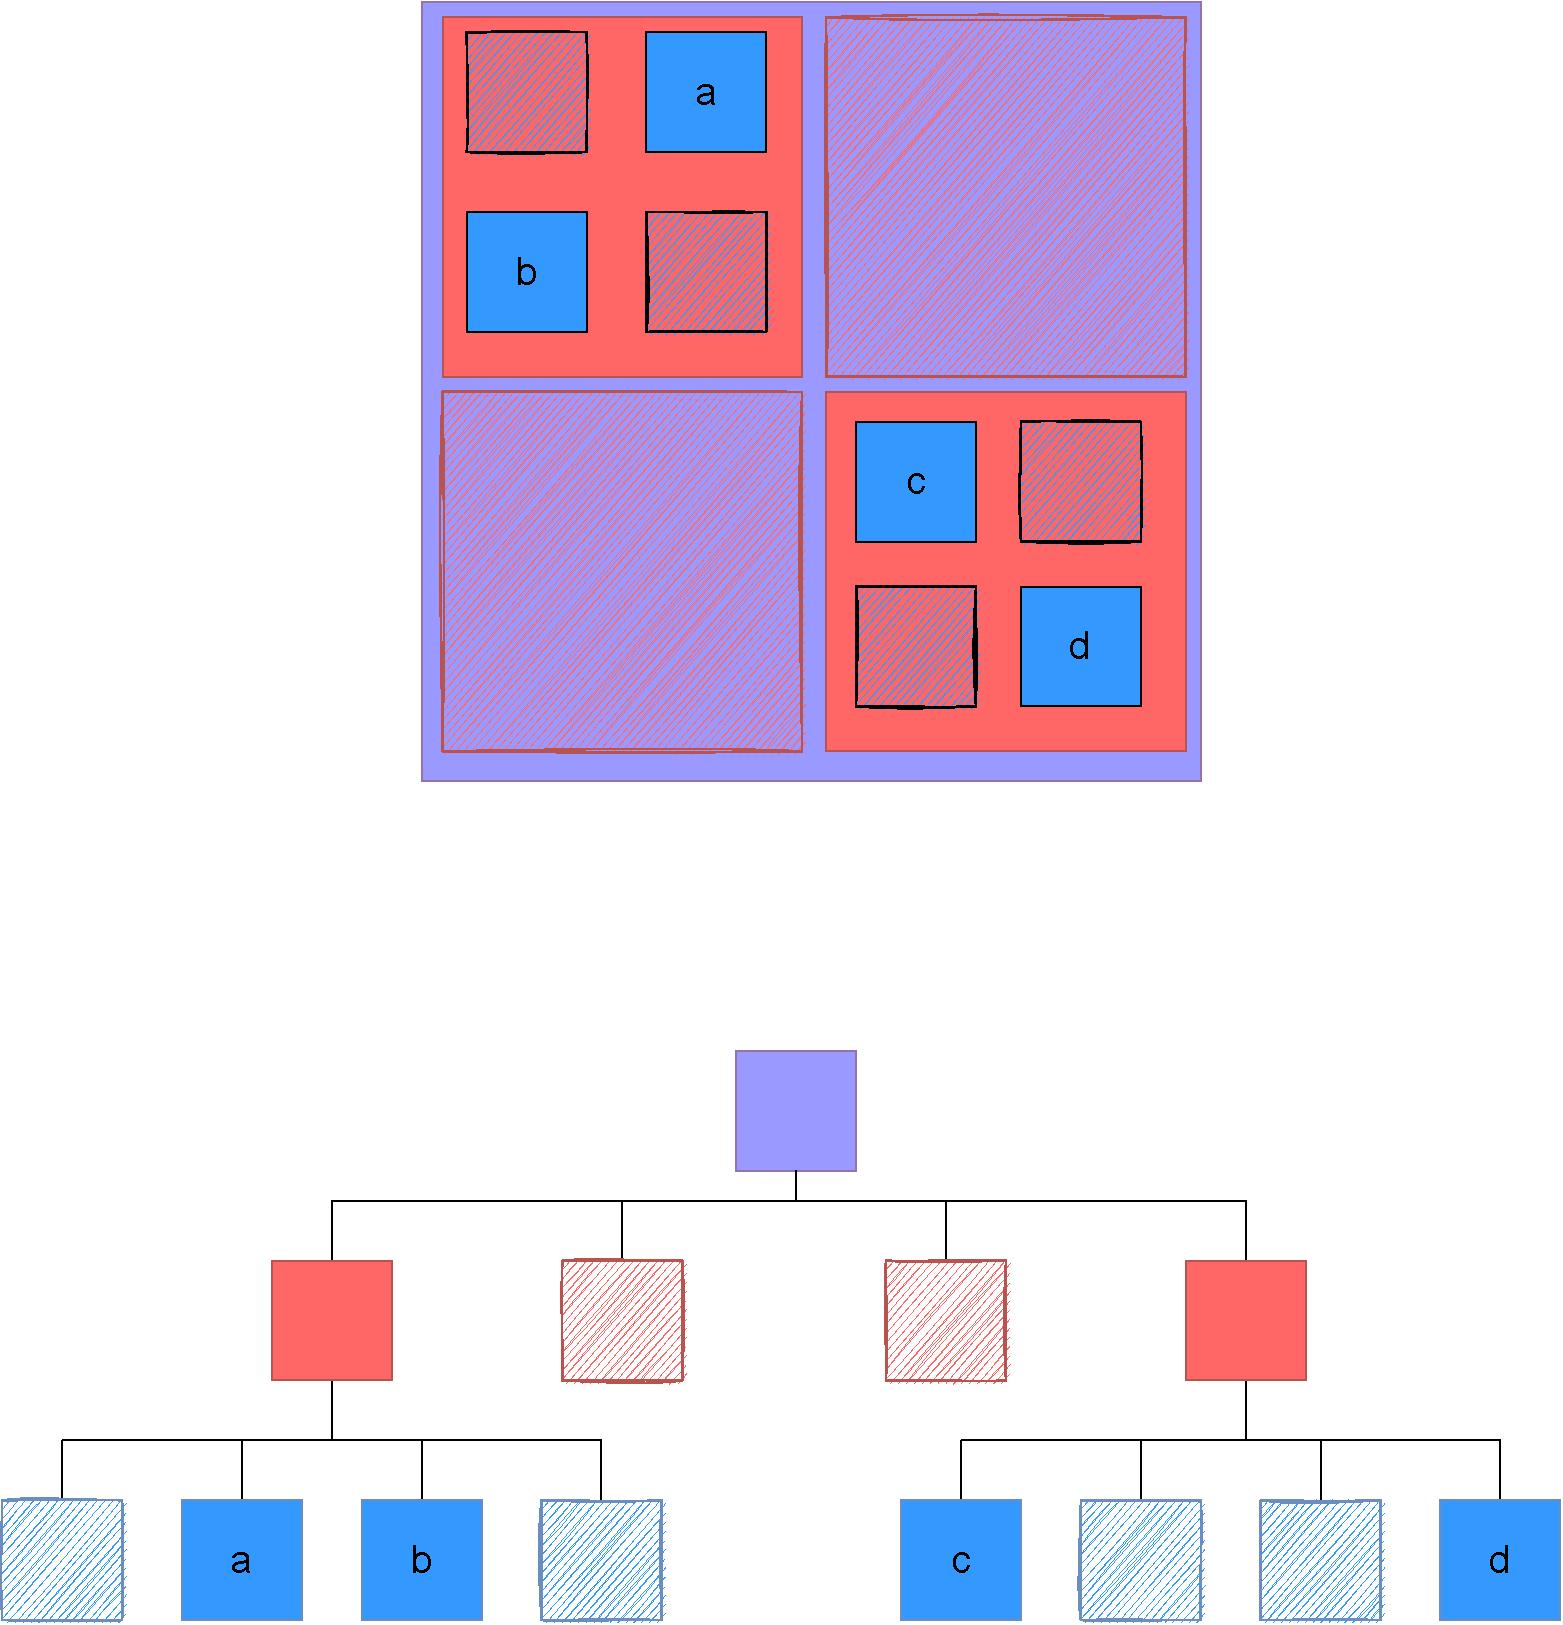
\includegraphics[width=0.8\textwidth]{figures/qtree.drawio.pdf}
    \caption{Quadtree representation}
    \label{fig:qtree}
\end{figure}

\subsection{GRIN}

Some other issues with FHW's frontend exist. FHW uses \textit{external core} representation of GHC, which was removed after GHC 7.6.3. This makes the compiler tightly coupled with Haskell, with the necessity to support various Haskell features, like type classes and burdens of primops. The obsolete version of GHC also makes the development process harder. FHW at the moment does not support partially applied functions in a frontend and CPS transformation is slow.

To mitigate the above issues, we opted for graph reduction intermediate notation  (GRIN)~\cite{GRIN} as a prospective frontend that would tie the frontend of the distiller and dataflow representation. It provides extra optimizations, like heap-points-to analysis, inlining, common subexpression elimination, etc., which improve the results of distillation: the distiller naively inlines some terms duplicating computations. 

All the essential frontend transformations of FHW are actually parts of the translation procedure into GRIN. The procedure includes variable names unification, variable lifting, lambda lifting,  and defunctionalization. These steps were implemented to translate a program from \texttt{.pot} language into \texttt{.grin}. \texttt{.pot} language does not allow recursive let bindings, which makes lambda lifting a bit easier. The algorithm could be found in~\cite{lambda-lift}. Defunctionalization is a part of the GRIN itself: the representation defines \texttt{ap}, \texttt{apply}, and \texttt{eval} procedures. The first one takes a function node and an argument node: it evaluates the function node and applies it to the argument. The second one operates with partially applied functions and constructors: it either saturates a function with one more argument or makes a function call if the argument fully saturates the function. The last one simply evaluates each possible node in a program.  These procedures are built during translation, when either a constructor application, or a function application (partial or saturated) are encountered. The notation is designed for lazy languages: it accumulates nodes without evaluating them if not needed, however the hardware is strict (otherwise, it would be needed to force node evaluation before transferring data from hardware to host). To make translated programs strict, calls to \texttt{eval} procedure are inserted to each function or constructor argument and functions are guaranteed to return and receive pointers to evaluated nodes. The implementation of the translator from \texttt{.pot} to \texttt{.grin} could be found at~\cite{grin-rep}.

GRIN representation uses static single assignment (SSA), and whilst SSA and CPS are equivalent~\cite{ssacps} they are different when generating hardware through dataflow. The current implementation is heavily CPS-depend\-ent, which makes control flow in dataflow straightforward: every recursive call is a tail call. This makes parallelization harder, since otherwise, chained recursive calls could be executed in parallel instead of chaining them with continuations. Such parallelization is more explicit in SSA form. However, SSA conversion into hardware would require heavy modifications to the current dataflow scheme and it is unclear whether it will maintain the existing formalisms that dataflow fulfills. Since CPS is crucial, to express it in GRIN several auxiliary routines are added and existing ones are modified: \texttt{eval} is modified to accept a continuation; \texttt{ap} applies a function to an argument in a continuation, which is passed to function evaluation; \texttt{apCont} is a version of \texttt{ap}, which accepts a continuation; \texttt{applyC} applies a partial function or constructor to an argument with continuation; \texttt{evalC} and \texttt{evalC2} are \texttt{eval} continuations for \texttt{ap} and \texttt{apCont} respectively. A full example for CPS transformation of a program, that adds to zeroes in Peano arithmetics could be seen on GitHub\footnote{\url{https://github.com/Tiltedprogrammer/SparseLinAlgHardware/blob/master/grin-examples/zero_plus_zero.grin} (online; accessed:
2022-06-07) Original program.}\textsuperscript{,}\footnote{\url{https://github.com/Tiltedprogrammer/SparseLinAlgHardware/blob/master/grin-examples/zero_plus_zero.grin.cps} (online; accessed:
2022-06-07) CPS-transformed program.}. 

Unfortunately, it appeared that heap-points-to analysis in the current implementation of GRIN worked only for tiny programs\footnote{\url{https://github.com/grin-compiler/grin/issues/128}  (online; accessed:
2022-06-07) A corresponding issue related to GRIN supporting only small enough programs.}, which is not the case for our sparse linear algebra routines. Since this analysis is crucial in GRIN, the prospective frontend was left until the analysis is performant enough and the part between GRIN and dataflow representation is unimplemented at the moment. 